\documentclass[12pt,a4paper]{report}

% --- Packages ---
\usepackage[utf8]{inputenc}
\usepackage[T1]{fontenc}
\usepackage{lmodern}
\usepackage[a4paper,margin=1in]{geometry}
\usepackage{setspace}
\usepackage{graphicx}
\usepackage{booktabs}
\usepackage{array}
\usepackage{amsmath, amssymb}
\usepackage{xcolor}
\usepackage{hyperref}
\usepackage{microtype}
\usepackage{listings}
\usepackage{caption}

\hypersetup{
  colorlinks=true,
  linkcolor=black,
  urlcolor=blue!60!black,
  citecolor=black,
  pdfborder={0 0 0}
}

\onehalfspacing

% --- Status markers (suppressed for final compile) ---
\newcommand{\status}[1]{}
\newcommand{\done}{}
\newcommand{\draftt}{}
\newcommand{\fillt}{}
\newcommand{\outlinet}{}

% --- Code listing style for shell / json blocks ---
\lstdefinestyle{plain}{
  basicstyle=\small\ttfamily,
  breaklines=true,
  columns=fullflexible,
  keepspaces=true,
  frame=single,
  framesep=4pt,
  backgroundcolor=\color{gray!5}
}
\lstset{style=plain}

% --- Title ---
\title{Adaptive Web Interaction:\\Leveraging Reinforcement Learning for Comprehensive Action Support}
\author{Muhammad Saad Ashraf \and Muhammad Salman Siddiq \and Awais Nazir}
\date{2026}

\begin{document}

% =========================================================
% TITLE PAGE
% =========================================================
\begin{titlepage}
  \centering
  \vspace*{1cm}
  {\Large \textbf{National University of Sciences and Technology (NUST)}\par}
  \vspace{0.4cm}
  {\large Pakistan\par}
  \vspace{2cm}
  {\Huge\bfseries Adaptive Web Interaction:\par}
  \vspace{0.3cm}
  {\LARGE Leveraging Reinforcement Learning\\ for Comprehensive Action Support\par}
  \vspace{2cm}
  {\large\itshape Final Year Project Report\par}
  \vspace{1.5cm}
  {\large Submitted by\par}
  \vspace{0.4cm}
  {\Large
    Muhammad Saad Ashraf\\[2pt]
    Muhammad Salman Siddiq\\[2pt]
    Awais Nazir\par
  }
  \vspace{1.5cm}
  {\large \textit{Supervisor:} Dr.~Faisal Shafait\par}
  \vfill
  {\large 2026\par}
\end{titlepage}

% =========================================================
% FRONT MATTER
% =========================================================
\pagenumbering{roman}

\chapter*{Certificate / Declaration}
\addcontentsline{toc}{chapter}{Certificate / Declaration}
Department-supplied templates. To be added during final compile.

\chapter*{Acknowledgments}
\addcontentsline{toc}{chapter}{Acknowledgments}

We thank our supervisor, Dr.~Faisal Shafait, for technical guidance and for the latitude to take this project in the direction the data ultimately demanded---toward the auditing of an existing benchmark rather than the introduction of a new one. We are grateful to the School of Electrical Engineering and Computer Science (SEECS) at the National University of Sciences and Technology for hosting this work and for the computing resources made available during initial exploration.

Outside of NUST, this project would not have been possible without the open release of the InSTA dataset and the \texttt{Insta-Qwen3-1.7B-SFT} checkpoint by Trabucco et~al., which we used as the starting point for both the audit and the RL training pipeline. We also acknowledge Google's GenAI free-tier credit programme, which subsidized the Vertex~AI Gemini~2.5~Flash judge calls that drove both the feasibility audit and the trajectory evaluation.

Finally, we thank our families and peers for their patience during the more compute-bound stretches of the project---an FYP that depends on a single GPU over several days exposes everyone in proximity to a steady hum and the occasional 3~AM checkpoint-restart.

\chapter*{Abstract}
\addcontentsline{toc}{chapter}{Abstract}
Browser-navigation benchmarks for web agents (InSTA, Mind2Web, WebArena) are widely used to evaluate small language models trained with reinforcement learning, but the websites they reference change continuously. We audit the InSTA-150k benchmark with a Gemini-based feasibility judge over 2{,}598 sampled test tasks and find that \textbf{only 28.3\% of tasks are reliably feasible}: 28.6\% target sites are inaccessible to automated agents, 13.0\% reference content that has since been removed or restructured, and 30.1\% are too uncertain for the judge to determine. We further show that \textbf{24.3\% of inaccessible sites returned an HTTP 2xx}, demonstrating that reachability probing alone is insufficient---semantic verification is required. We then apply PPO + LoRA reinforcement-learning training to the base SFT model on a 2{,}068-task feasibility-filtered subset and evaluate on a 100-task held-out feasibility-filtered test set. RL training on the cleaned subset yields \textbf{a +17.1 percentage-point improvement in mean judge-success score (from 29.05\% for the base SFT model to 46.17\% for the RL-trained checkpoint)}, suggesting that benchmark hygiene materially affects measured agent performance.

\tableofcontents
\listoffigures
\listoftables

% =========================================================
% MAIN BODY
% =========================================================
\clearpage
\pagenumbering{arabic}

% ---------- Chapter 1 ----------
\chapter{Introduction}

\section{Background and Motivation}

Small language models (SLMs) fine-tuned for browser navigation are an active area of research, with reinforcement learning increasingly used to improve agent behavior beyond what supervised fine-tuning alone can achieve. A typical pipeline trains an SLM agent against a benchmark of natural-language tasks, each grounded in a specific live website (e.g.~\textit{``find the price of an iPhone~15 on apple.com''}). The agent's actions---clicks, form fills, navigations---are evaluated by a separate LLM judge that scores the resulting trajectory on success, efficiency, and self-correction.

This pipeline rests on a quiet assumption: \textbf{the benchmark tasks remain valid over time}. That is, the websites they reference still respond, the content the task asks about still exists, and the navigation steps still resolve to the right answer. In practice, this assumption breaks rapidly. Sites disappear, redirect, deploy bot-detection, restructure content, or simply update---all without notice to anyone training agents against them. When a substantial fraction of ``the benchmark'' is silently broken, the gap between the agent's capability and its measured performance is no longer just a function of the agent: it is a compound of the agent's ability and the benchmark's residual usability. Training signal computed against broken tasks is at best noise and at worst a directly counter-productive gradient.

The motivating question for this project is therefore not ``how do we train a better web agent?'' but ``what fraction of our training and evaluation budget is being wasted on tasks that no model could possibly succeed at, and what happens when we remove them?''

\section{Problem Statement}

Existing reinforcement-learning pipelines for browser-navigating language models train and evaluate against fixed snapshots of the live web. Over time these snapshots drift: websites change, become inaccessible to automated agents, or have their content removed. Despite this widely-acknowledged practical problem, no published work systematically audits a popular web-agent benchmark to quantify the rate and nature of this decay, and no public training pipeline filters out broken tasks before they are used to compute training reward. As a result, both reported agent performance and the agent itself are confounded by benchmark hygiene effects of unknown magnitude.

\section{Objectives}

The objectives of this project, in order of dependency, are:
\begin{enumerate}
  \item Quantify the feasibility decay of the InSTA-150k web-agent benchmark by classifying a representative sample of its tasks using a Gemini-2.5-Flash-based judge with URL-context grounding.
  \item Construct two reusable artifacts from the audit: (a) a feasibility-filtered \emph{training} subset that excludes broken tasks, and (b) a feasibility-filtered \emph{held-out test} subset usable for unbiased evaluation.
  \item Train a small (1.7~B parameter) language-model agent on the cleaned training subset using PPO with LoRA adapters, anchored to the base SFT policy via a reference-KL term.
  \item Evaluate the trained agent against the unmodified base SFT model on the held-out filtered set, using paired statistical tests (Wilcoxon and McNemar) to quantify the gap.
  \item Release reproducibility artifacts---code, per-task feasibility classifications, hyperparameters, and the trained checkpoint---under a public GitHub repository so that any reviewer or follow-on researcher can re-run the evaluation end-to-end.
\end{enumerate}

\section{Scope and Assumptions}

\paragraph{In scope.} The InSTA-150k benchmark serves as the single subject of audit and training; we do not experimentally generalize to other web-agent benchmarks (WebArena, Mind2Web, WebShop) but discuss them in the literature review and use the same methodology where applicable. The agent is the publicly available \texttt{btrabucco/Insta-Qwen3-1.7B-SFT} checkpoint at a single model size. Hardware is one NVIDIA L4 (24~GB VRAM) provisioned on Google Cloud Platform. Both the feasibility judge and the trajectory judge are Gemini~2.5~Flash, accessed through Vertex AI. Browser automation is performed via a Playwright server with a headless Chromium back-end.

\paragraph{Out of scope.} We do not train Qwen from scratch---the project fine-tunes an already-supervised model. We do not study multi-agent setups or human-in-the-loop training. The agent operates only on web pages rendered as HTML/Markdown observations: mobile-app, native-application, and vision-language navigation are excluded. Larger models (above $\sim$2~B parameters) and distributed multi-GPU training are also excluded.

\paragraph{Assumptions.} The audit assumes that the websites referenced by InSTA-150k remain sufficiently stable over the audit's wall-clock window (a few days) to give consistent classifications. We assume that Gemini~2.5~Flash's classification behavior is reproducible across calls within the project window: a small sanity-check sample (Appendix~\ref{app:sanity-check}) provides spot evidence for this. We assume the InSTA-provided train/test split is appropriate and do not re-split. Finally, the experimental design assumes that single-trajectory PPO updates---necessary given our compute budget---are sufficient to surface measurable performance differences if they exist; any null results are interpreted with this caveat in mind.

\section{Contributions}

This project makes two contributions:

\begin{enumerate}
  \item \textbf{A feasibility audit of the InSTA-150k benchmark.} We use a Gemini-2.5-Flash-based judge with URL-context grounding to classify 2{,}598 sampled InSTA test tasks into four categories---feasible, website-down, content-outdated, uncertain. We report per-class breakdowns, characterize the disagreement between cheap HTTP-reachability probes and the more expensive LLM judge, and release the per-task classifications for reuse.
  \item \textbf{An RL training experiment on a feasibility-filtered subset.} We apply PPO + LoRA training to the base SFT model on a 2{,}068-task feasibility-filtered training subset, and evaluate on a 100-task held-out feasibility-filtered subset, comparing the trained model against the base SFT baseline.
\end{enumerate}

Our results suggest that benchmark hygiene is not just a measurement issue but an \textbf{agent-development} issue: training on a set of mostly-broken tasks corrupts the gradient signal, while training on a cleaned subset produces a measurably better agent.

\section{Report Organization}

Chapter~\ref{chap:litreview} surveys prior work on web-agent benchmarks, reinforcement learning for language models, parameter-efficient fine-tuning, and LLM-as-judge evaluation, and positions our contributions against the gap analysis of those literatures. Chapter~\ref{chap:methodology} describes the three pipelines that constitute the work---the feasibility audit, the RL training loop, and the held-out evaluation methodology---together with the reward design and the PPO update equations. Chapter~\ref{chap:implementation} translates the methodology into code: software architecture, GCP infrastructure, the Playwright watchdog, and the reproducibility artifacts shipped with the project. Chapter~\ref{chap:results} presents the results: the feasibility-audit numbers and Figure~1 (\S\ref{sec:feasibility-results}), the training dynamics, the headline held-out evaluation comparison, and a discussion of what the numbers do and do not support. Chapter~\ref{chap:conclusion} concludes with limitations and future work. Appendices contain the sanity-check sample, exact reproducibility commands, the hyperparameter table, and the per-experiment compute footprint.

% ---------- Chapter 2 ----------
\chapter{Literature Review}\label{chap:litreview}

This chapter surveys the literatures most directly relevant to the project: web-agent benchmarks (\S\ref{sec:lit-webagents}), reinforcement learning for language models (\S\ref{sec:lit-rl}), parameter-efficient fine-tuning (\S\ref{sec:lit-peft}), LLM-as-judge evaluation (\S\ref{sec:lit-judge}), the benchmark we audit specifically (\S\ref{sec:lit-insta}), and the smaller but growing literature on benchmark integrity and dataset decay (\S\ref{sec:lit-decay}). Section~\ref{sec:lit-gap} positions our two contributions against the gap that this combined survey reveals.

\section{Web Agents and Browser Automation}\label{sec:lit-webagents}

The recent surge of interest in web-navigating language-model agents traces back to two threads: a reformulation of web tasks as natural-language goals coupled with structured action spaces, and a series of benchmarks that operationalize that reformulation at scale.

\textbf{WebShop}~\cite{yao2022webshop} introduced one of the first widely-used web-agent benchmarks. The agent shops on a simulated e-commerce site to fulfil natural-language product requests; success is judged by attribute matching against a target product. WebShop's defining choice was to use a \emph{simulated} environment with a fixed snapshot of product data, eliminating live-web non-determinism but at the cost of distributional realism.

\textbf{Mind2Web}~\cite{deng2023mind2web} took the opposite approach: it scraped 2{,}350 tasks across 137 real websites and 31 domains, and recorded human demonstrations of each task. Mind2Web is closer to the deployment distribution, but its evaluation is offline (compare predicted action to recorded demonstration), so it cannot measure end-to-end task success on a still-live site.

\textbf{WebArena}~\cite{zhou2023webarena} attempted to combine the realism of real websites with end-to-end success-rate evaluation by running its own self-hosted clones of five common web-app categories (e-commerce, forums, gitlab, etc.). Self-hosting solves the staleness problem but requires the benchmark authors to maintain server infrastructure indefinitely. \textbf{VisualWebArena}~\cite{koh2024visualwebarena} extends this with vision-grounded variants of the same tasks.

\textbf{AgentBench}~\cite{liu2023agentbench} is a meta-benchmark that aggregates eight distinct agent tasks (including web navigation) into a single evaluation suite, with a focus on comparing closed-source and open-source LLM agents under a uniform protocol.

\textbf{InSTA}~\cite{trabucco2025insta}---the subject of our audit---takes yet another tack. It scales to 150{,}000 tasks across 100{,}000+ live websites by using an LLM-driven task-generation pipeline rather than human annotation, and ships an SFT'd Qwen3-1.7B agent trained on the resulting trajectories. The combination of scale, public availability of both data and model, and live-web execution makes InSTA particularly suitable for a feasibility audit: it is large enough that decay can be measured statistically, public enough that the audit's results are independently verifiable, and live enough that decay is non-trivial.

The recurring methodological tension in this literature is between \emph{realism} (test on the live web) and \emph{stability} (use a fixed snapshot or self-hosted clone). InSTA chose realism. Our project measures the cost of that choice.

\section{Reinforcement Learning for Language Models}\label{sec:lit-rl}

Reinforcement learning has become the dominant paradigm for steering large language models beyond what supervised fine-tuning can achieve. The relevant ideas, in chronological order:

\textbf{PPO}~\cite{schulman2017ppo} (Proximal Policy Optimization) is the workhorse on-policy algorithm of modern LLM RL. It optimizes a clipped surrogate objective that approximates a constrained policy update without explicitly solving a trust-region problem at each step. The clipping mechanism in particular is what makes PPO numerically tractable on the high-dimensional action spaces that token-level language modeling implies.

\textbf{RLHF}~\cite{ouyang2022instructgpt} (Reinforcement Learning from Human Feedback) was popularized by InstructGPT and uses PPO with a learned reward model that approximates human preferences. The recipe is: (1)~SFT on instruction-response pairs, (2)~train a reward model on human preference labels, (3)~PPO against that reward, with a KL penalty against the SFT model to prevent drift. The KL penalty is now standard.

\textbf{RLAIF}~\cite{bai2022constitutional} (Constitutional AI / RL from AI Feedback) replaces the human preference labeler with another LLM, dramatically reducing the cost of label collection. Our project's use of Gemini~2.5~Flash as the trajectory judge sits in this lineage: the judge is an LLM, not a human annotator, but the structural role---providing the scalar reward signal---is the same.

\textbf{GRPO}~\cite{shao2024deepseekmath} (Group Relative Policy Optimization) drops the value-function critic that classical PPO uses and instead computes advantages from intra-group reward differences (multiple sampled responses per prompt). This sidesteps the value-function-fitting overhead and has become popular for code- and math-reasoning RL.

\textbf{RLOO}~\cite{ahmadian2024rloo} (REINFORCE Leave-One-Out) revisits classical REINFORCE with a leave-one-out baseline computed from sibling samples. Like GRPO, it dispenses with a learned value function. The headline finding is that, on RLHF-style problems, simple REINFORCE-with-baseline matches or exceeds PPO at lower implementation complexity.

The choice of algorithm in the present project is PPO with a reference-policy KL anchor (\S\ref{sec:ppo-update}), not GRPO or RLOO, for two reasons: (a)~the trajectory length in web navigation (up to 20 steps with multi-token actions per step) makes the per-trajectory cost of group-relative methods prohibitive on a single L4, and (b)~the reference-KL anchor we add to PPO addresses the long-horizon drift problem in a way GRPO does not (GRPO's anchoring is only within a group, not against the SFT model).

\section{Parameter-Efficient Fine-Tuning}\label{sec:lit-peft}

Parameter-efficient fine-tuning (PEFT) techniques replace full-parameter updates with low-cost auxiliary parameters that mediate the model's behaviour, leaving the base weights frozen. The key methods, ordered by influence on contemporary practice:

\textbf{Adapters}~\cite{houlsby2019adapters} insert small bottleneck networks between transformer sub-layers and train only those. They were the first widely-adopted PEFT technique but were superseded for most use cases by lighter-touch alternatives.

\textbf{Prefix tuning}~\cite{li2021prefix} prepends learnable vectors to the input sequence at each transformer layer; only those vectors are trained. The compute footprint is small but the optimization dynamics are notoriously fragile.

\textbf{LoRA}~\cite{hu2021lora} (Low-Rank Adaptation) is the dominant PEFT method in LLM RL. It re-parameterizes each weight matrix update as the product of two low-rank factors, $\Delta W = BA$, where $A \in \mathbb{R}^{r \times d}$ and $B \in \mathbb{R}^{d \times r}$ for a small rank $r$. Crucially, $A$ is initialized randomly (Gaussian) and $B$ is initialized at zero, so the adapted model starts behaviourally identical to the base. We use LoRA with $r=8$ throughout, on the attention projection matrices.

\textbf{IA3}~\cite{liu2022ia3} introduces three learnable vectors per layer that gate the keys, values, and the FFN output. The parameter count is even smaller than LoRA but the expressive capacity is also lower; on RL-style tasks LoRA tends to perform better.

\textbf{QLoRA}~\cite{dettmers2023qlora} combines LoRA with 4-bit NF4 quantization of the base weights, double quantization of the quantization constants, and paged optimizers. The result is that a 7--65~B-parameter model can be PEFT-fine-tuned on a single consumer GPU. We adopt QLoRA's NF4 + double-quant + bfloat16-compute recipe directly: it is what makes 1.7~B-parameter PPO + LoRA feasible on a single 24~GB L4.

\section{LLM-as-Judge Evaluation}\label{sec:lit-judge}

Using one language model to evaluate another's outputs has emerged as the dominant alternative to crowd-sourced human evaluation. The core attractions are scale (judges run hundreds of times faster than annotators) and consistency (a single model judging at fixed temperature is more reproducible than a panel of humans).

\textbf{G-Eval}~\cite{liu2023geval} formalizes the LLM-as-judge protocol with a chain-of-thought-prompted evaluator and reports correlations with human judgments above 0.5 on summarization tasks. \textbf{Chatbot Arena}~\cite{zheng2023chatbot} and \textbf{AlpacaEval}~\cite{li2023alpacaeval} adapt the protocol to head-to-head model comparison and pairwise preference, respectively.

The reliability of LLM judges has been actively investigated. Wang et~al.~\cite{wang2023largejudge} document a substantial \emph{position bias}: LLM judges presented with two responses prefer the first in some configurations and the second in others, with the bias often dominating the genuine quality signal. Mitigations include randomized order, score-based rather than preference-based prompts, and ensembles across judge models.

For our project, the judge plays two roles. In the feasibility audit (\S\ref{sec:feasibility-pipeline}), Gemini~2.5~Flash uses its \texttt{url\_context} tool to ground its classification in the page's actual current state, and returns a four-way categorical decision rather than a numeric score---reducing one degree of freedom for bias to operate through. In the trajectory evaluation (\S\ref{sec:eval-method}), the judge returns three component scalars rather than a pairwise preference, which avoids position-bias entirely (only one trajectory is shown per prompt). We do not separately calibrate the judge against human labels, which is a limitation discussed in \S\ref{sec:limitations}.

\section{The InSTA Benchmark in Detail}\label{sec:lit-insta}

InSTA~\cite{trabucco2025insta} is the largest publicly available web-navigation benchmark by task count: 150{,}000 (instruction, website) pairs spanning 100{,}000+ unique websites. The pipeline that produces these tasks runs entirely with LLMs:
\begin{enumerate}
  \item A seed web-search query generates a candidate URL.
  \item A planner LLM proposes one or more navigation tasks plausibly supported by that URL.
  \item A verifier LLM filters out tasks that the page state cannot support.
  \item A demonstrator LLM produces a reference trajectory for accepted tasks.
\end{enumerate}

The output is a (\texttt{website}, \texttt{instruction}, \texttt{steps}, \texttt{criteria}) tuple per task, where \texttt{steps} is the demonstrator's plan and \texttt{criteria} is the verifier's success rubric. The benchmark ships with two SFT models (Qwen2.5-1.5B and Qwen3-1.7B) trained on the demonstrator trajectories.

InSTA is well-suited to the questions we ask in this project for three reasons. First, it is large enough that subsampling 2{,}598 tasks for the feasibility audit is statistically meaningful while still tractable to score with a paid judge. Second, both the data and the agent are public, making any audit and any RL fine-tuning result independently verifiable. Third, the live-web execution model means decay is measurable: a task generated against a website in early 2025 may visit a substantially different page in late 2026, and the gap is precisely what our audit quantifies.

\section{Benchmark Integrity and Dataset Decay}\label{sec:lit-decay}

Despite the centrality of benchmarks in modern ML, the literature on \emph{benchmark integrity}---auditing existing benchmarks for problems---is comparatively thin.

The closest body of work is on \textbf{data contamination} in language-model evaluation: cases where evaluation data has leaked into training corpora. Dodge et~al.~\cite{dodge2021c4} document the contents of C4 and find that several common evaluation sets are partially included in the pretraining data. Magar and Schwartz~\cite{magar2022contamination} propose probing techniques to estimate the extent of memorization-based score inflation.

For \textbf{web-agent benchmarks specifically}, no published audit (as of writing) systematically measures the rate at which benchmark tasks become inexecutable due to website changes. The closest references are anecdotal: WebArena's authors note in their paper that self-hosting is necessary precisely because live-web tasks decay; the InSTA paper does not benchmark the issue but acknowledges it.

In \textbf{adjacent domains}, dataset decay has been documented for: news-headline classification (where label distributions shift as news cycles change), recommender-system benchmarks (where catalog turnover invalidates ground truth), and software-engineering benchmarks based on GitHub issues (where issues get closed and code refactored). The methodological idea that ``a benchmark with a non-trivial fraction of broken items will systematically under-report agent capability'' is implicit in these literatures but has not, to our knowledge, been quantitatively tied to a specific live-web benchmark.

\section{Gap Analysis and Positioning}\label{sec:lit-gap}

Reading these literatures together, two complementary gaps emerge.

\textbf{First}, the web-agent benchmark literature (\S\ref{sec:lit-webagents}) has resolved the realism-stability tension in two ways: by self-hosting (WebArena) or by going offline (Mind2Web). Live-web benchmarks like InSTA have not been systematically audited for decay, even though decay is the precise reason WebArena chose self-hosting in the first place. Our \S\ref{sec:feasibility-results} contribution fills this gap directly: a quantitative audit of one specific live-web benchmark, with per-class breakdown, methodology described in enough detail to be replicated against other benchmarks, and per-task classifications released publicly.

\textbf{Second}, the RL-for-LLM literature (\S\ref{sec:lit-rl}) has paid heavy attention to algorithmic improvements (PPO~$\to$~GRPO~$\to$~RLOO) and to KL-anchoring techniques, but has paid little attention to the data side: \emph{is the gradient signal we are optimizing actually meaningful?} This project does not propose a new RL algorithm; instead it proposes that data hygiene is a complementary axis along which agent capability can be improved. Our \S\ref{sec:rl-training} contribution makes this concrete by training the same algorithm (PPO + LoRA + reference-KL anchor) on a feasibility-filtered subset, and the held-out evaluation in \S\ref{sec:eval-method} measures whether the data improvement carries through to measured capability.

The positioning, then, is: existing work either trains on raw web benchmarks (assuming the data is sound) or builds new benchmarks (a one-off audit at construction time only). No published work, as far as we can establish, audits an existing public benchmark for decay \emph{and} re-runs RL training on a controlled cleaned subset. This project does both, and ties the two contributions together via a paired held-out evaluation.

% ---------- Chapter 3 ----------
\chapter{Methodology}\label{chap:methodology}

\section{Overall Approach}

The methodology comprises three coupled pipelines that share a common agent (Qwen3-1.7B-SFT), a common LLM judge (Gemini~2.5~Flash via Vertex~AI), and a common reward formulation. The pipelines compose linearly: the feasibility audit (\S\ref{sec:feasibility-pipeline}) produces a cleaned task pool from which both a training subset (consumed by \S\ref{sec:rl-training}) and a held-out test subset (consumed by \S\ref{sec:eval-method}) are drawn. The RL training pipeline runs the agent online against the live web, gathers trajectories, scores them with the judge, and updates the LoRA adapter via PPO with a reference-policy anchor. The held-out evaluation pipeline runs the same agent (with and without the LoRA adapter) on the previously-unseen test subset and produces paired statistical comparisons.

The advantage of this layout is that the same judge serves three different roles---feasibility classification, training-time reward, and evaluation-time scoring---so any judge-specific systematic bias affects all three measurements equally and tends to cancel in pairwise comparisons. The disadvantage is that all three rely on Gemini~2.5~Flash being available and behaving consistently throughout the project window, a dependency we discuss further in \S\ref{sec:limitations}.

\section{Feasibility Audit Pipeline}\label{sec:feasibility-pipeline}

For each candidate task $(w, q)$ where $w$ is the target website URL and $q$ the natural-language instruction, we run a two-stage feasibility check:

\begin{enumerate}
  \item \textbf{HTTP probe.} A simple \texttt{requests.get(w, timeout=10)} retrieves the response status and any reachability error. This is bounded and fast (\textasciitilde 200~ms / task) and acts as a coarse filter.
  \item \textbf{LLM judge with URL-context grounding.} A Gemini-2.5-Flash model is prompted with the task instruction, the HTTP probe result, and today's date; it is given a \texttt{url\_context} tool that lets it actually fetch and inspect the target page. The judge returns a JSON object:
  \begin{lstlisting}
{"classification": one of {FEASIBLE, WEBSITE_DOWN,
                           CONTENT_LIKELY_OUTDATED, UNCERTAIN},
 "confidence": [0, 1],
 "reasoning": str}
  \end{lstlisting}
  We classify a task as \textbf{feasible} if and only if the judge returns \texttt{FEASIBLE} with confidence $\geq 0.95$. The strict threshold trades sample size for precision.
\end{enumerate}

The judge prompts the model to consider:
\begin{itemize}
  \item whether the site is reachable from the model's URL-context tool,
  \item whether any page on the site is likely to contain the answer to $q$,
  \item whether the navigation steps implied by $q$ are still completable on the current site,
  \item whether the date suggests the content might be stale.
\end{itemize}

This combined HTTP + LLM-judge methodology surfaces failures that neither method alone catches.

\section{RL Training Pipeline}\label{sec:rl-training}

Our agent is \texttt{btrabucco/Insta-Qwen3-1.7B-SFT}---a Qwen3-1.7B model already supervised-fine-tuned on InSTA web-navigation trajectories---quantized to 4-bit (NF4 with double quantization) at inference and training time. We attach a LoRA adapter ($r=8$, $\alpha=16$, dropout$=0.05$; targets attention projections), giving 17.4~M trainable parameters out of 1.03~B (1.69\%).

Each trajectory:
\begin{enumerate}
  \item Initializes a new Playwright browser session at the task's target URL.
  \item Iterates up to 20 (observation, action) steps, where each step:
    \begin{itemize}
      \item converts the current page to Markdown via the InSTA pipeline,
      \item constructs a prompt from the instruction, current observation, and last 2 history turns,
      \item generates an action JSON via the model (\texttt{max\_new\_tokens=512}, temperature$=0.7$, top-p$=0.9$),
      \item parses the action and executes it in the browser,
      \item receives the next observation.
    \end{itemize}
  \item Terminates either via a \texttt{stop} action emitted by the agent or after 20 steps.
  \item Sends the full trajectory to the judge, which returns $(\text{success}, \text{efficiency}, \text{self\_correction}) \in [0, 1]^3$.
\end{enumerate}

\section{Reward Design and PPO Update}\label{sec:ppo-update}

The reward is the convex combination
\begin{equation}
  R = 0.7 \cdot \text{success} + 0.2 \cdot \text{efficiency} + 0.1 \cdot \text{self\_correction} \in [0, 1].
\end{equation}

For each completed trajectory $\tau = \{(s_t, a_t)\}_{t=0}^{T-1}$, we compute three sets of step-wise log-probabilities:
\begin{itemize}
  \item $\log \pi_\text{old}(a_t \mid s_t)$---the policy at the start of this update (no gradient).
  \item $\log \pi_\text{ref}(a_t \mid s_t)$---the base SFT policy (LoRA disabled), no gradient. Computed every 5th update for efficiency.
  \item $\log \pi_\text{new}(a_t \mid s_t)$---the current policy with gradient tracking.
\end{itemize}

The PPO loss combines a clipped surrogate, an entropy bonus, and \textbf{two} KL penalties:
\begin{equation}
\begin{split}
  \mathcal{L} = -\min\!\big( r_t A_t,\; \text{clip}(r_t, 1-\varepsilon, 1+\varepsilon) A_t \big) - \beta_H\,\mathcal{H}[\pi_\text{new}] \\
              + \beta_\text{KL}\,D_\text{KL}(\pi_\text{new} \,\|\, \pi_\text{old}) + \beta_\text{ref}\,D_\text{KL}(\pi_\text{new} \,\|\, \pi_\text{ref})
\end{split}
\end{equation}
with $r_t = \exp(\log \pi_\text{new} - \log \pi_\text{old})$, $\varepsilon = 0.1$, $\beta_H = 0.01$, $\beta_\text{KL} = 0.1$, $\beta_\text{ref} = 0.05$. Gradients are clipped to a max norm of 0.5 before an AdamW step at learning rate 2$\times 10^{-5}$. We use a single PPO epoch per trajectory; training proceeds online.

The reference-KL term anchors the LoRA-updated policy to the base SFT model's distribution, preventing cumulative drift over many trajectories that the within-trajectory PPO clip would not catch.

\section{Trajectory Rollout via Playwright}\label{sec:rollout}

The agent does not interact with websites directly; it does so through a long-running Playwright server that we operate alongside the Python trainer. The split-process design (Python policy + Node.js browser server) is dictated by Playwright's API surface being native to JavaScript and by the practical need to keep browser-state lifecycle independent of training-loop restarts.

\subsection*{Server architecture}

A Node.js process exposes a small HTTP surface on \texttt{localhost:3000} with three core endpoints: \texttt{POST /start} opens a new headless Chromium context and returns a session identifier; \texttt{POST /goto} navigates that session to a URL; \texttt{POST /action} executes a list of Playwright function calls (clicks, scrolls, form fills, etc.) addressed by a custom \texttt{backend\_node\_id} attribute that the InSTA observation pipeline injects into rendered HTML. The server is single-threaded but operates one Chromium context per session, so multiple trajectories could in principle be parallelized---a future-work item.

\subsection*{Per-step loop}

For a single trajectory, the Python trainer:
\begin{enumerate}
  \item Calls \texttt{/start} to allocate a fresh browser session, then \texttt{/goto} to load the task's target URL.
  \item Polls the page for an \emph{observation}: the raw HTML, plus per-element metadata (visibility, role, accessibility name) computed by the InSTA observation pipeline.
  \item Converts the HTML+metadata to a structured Markdown representation that fits within the agent's prompt budget (the \texttt{markdown} module of the InSTA package).
  \item Constructs a prompt from the task instruction, the current Markdown observation, and the last two history turns.
  \item Generates an action JSON via the (LoRA-adapted) Qwen3-1.7B model under sampling parameters \texttt{(temperature=0.7, top\_p=0.9, max\_new\_tokens=512)}.
  \item Parses the JSON, dispatches it to \texttt{/action}, and waits for the next observation. The loop terminates after at most 20 steps, or earlier if the agent emits an action with \texttt{action\_key} of \texttt{stop}.
\end{enumerate}

\subsection*{The watchdog}

Because each trajectory is a long, stateful interaction with a real website, transient failures of the Playwright server (browser crashes, network hiccups, Chromium memory bloat) will cascade into many failed trajectories if not handled. A separate \texttt{playwright\_watchdog.sh} process polls port~3000 every 20 seconds. When the server is unreachable, the watchdog (a)~sends \texttt{SIGSTOP} to the Python trainer to pause learning before it consumes a malformed observation, (b)~kills the stale server, (c)~restarts a fresh server, (d)~waits for it to respond on \texttt{/start}, and (e)~sends \texttt{SIGCONT} to the trainer to resume. The trainer treats the resumed step as a normal observation and proceeds. This recovery loop adds approximately 30~seconds of wall-time per outage but converts an outage from ``many failed trajectories'' into ``one short pause''.

\section{Held-out Evaluation Methodology}\label{sec:eval-method}

The evaluation answers a single, paired question: \emph{does an agent with our LoRA adapter outperform the unmodified base SFT model on a held-out feasibility-filtered task set?} The methodology is designed to give that question a defensible quantitative answer despite the inherent stochasticity of an LLM agent and an LLM judge.

\subsection*{Paired design}

Both arms (the LoRA-adapted ``RL-on-filtered'' checkpoint and the unmodified ``Base SFT'' model) are evaluated on \emph{the same} 100 tasks, sampled from the held-out test CSV with a fixed pseudo-random seed (42). Same tasks $\to$ paired comparison: the differences between matched per-task rewards are the relevant statistic. We do not compare independent samples because the per-task variance dominates the per-arm variance, so unpaired tests would be needlessly under-powered.

The \texttt{--compare} flag in \texttt{evaluate\_checkpoint.py} runs both arms in sequence within a single process: first the LoRA-adapted checkpoint, then the base model with adapters disabled (via PEFT's \texttt{disable\_adapter\_layers}). Same agent, same prompt-construction, same judge, same per-step temperature---only the LoRA delta to the policy weights changes between arms.

\subsection*{Per-task reward and binary success}

For each task the judge returns three component scores in $[0, 1]$: \texttt{success}, \texttt{efficiency}, and \texttt{self\_correction}. From these we derive two per-task quantities:
\begin{itemize}
  \item the \emph{composite reward} $R = 0.7\,\text{success} + 0.2\,\text{efficiency} + 0.1\,\text{self\_correction}$, matching the training reward formulation in \S\ref{sec:ppo-update}; and
  \item a \emph{binary success indicator} $\mathbb{1}[\text{success} > 0.5]$, used for the McNemar paired test.
\end{itemize}

\subsection*{Statistical analysis}

Three statistics are reported for the paired comparison:
\begin{enumerate}
  \item \textbf{Mean delta with 95\% bootstrap CI.} For both reward and binary success, we compute the mean per-task difference between the two arms and a 95\% percentile bootstrap CI (10{,}000 resamples, fixed bootstrap seed 0). The CI's distance from zero is the operationally important quantity.
  \item \textbf{Paired Wilcoxon signed-rank test} on the per-task reward delta. This is the non-parametric paired test of choice when reward is continuous and not Gaussian.
  \item \textbf{McNemar exact test} on the binary success indicator. This is the paired test for paired binary outcomes; we report the exact (not chi-squared) variant given the small expected discordant counts.
\end{enumerate}

The \texttt{eval/analyze\_eval\_results.py} script consumes the per-arm JSONs that \texttt{evaluate\_checkpoint.py --compare} writes (\texttt{checkpoint\_results\_*.json}, \texttt{base\_results\_*.json}), produces a Markdown table and a CSV summary, and renders Figure~3 (a 2-bar comparison with bootstrap-CI error bars). It also writes a compact \texttt{summary.json} for downstream consumption.

% ---------- Chapter 4 ----------
\chapter{Implementation}\label{chap:implementation}

This chapter translates the methodology of Chapter~\ref{chap:methodology} into the actual software artefact submitted with this report. The presentation is organized by concern: software architecture (\S\ref{sec:impl-arch}), the cloud infrastructure that hosts training and evaluation runs (\S\ref{sec:impl-gcp}), the Playwright server's watchdog (\S\ref{sec:impl-watchdog}), the code-base layout (\S\ref{sec:impl-code}), and finally the reproducibility artefacts shipped for reviewers (\S\ref{sec:impl-repro}).

\section{Software Architecture}\label{sec:impl-arch}

The system is split across three processes that communicate over the loopback interface:
\begin{itemize}
  \item A \textbf{Python trainer / evaluator} that holds the model weights, runs the policy forward and backward passes, and orchestrates the per-trajectory rollout loop. The two entry points are \texttt{pipeline\_in\_steps.py} (training) and \texttt{evaluate\_checkpoint.py} (held-out evaluation); both share the same internal modules under \texttt{src/}.
  \item A \textbf{Node.js Playwright server} that owns the browser sessions and exposes a small HTTP surface on \texttt{localhost:3000} for starting sessions, navigating, and dispatching actions. This is the same server used by the InSTA reference implementation.
  \item An \textbf{external Vertex AI Gemini~2.5~Flash endpoint} that answers two distinct prompt types: feasibility-classification prompts (during the audit) and trajectory-judgment prompts (during training and evaluation).
\end{itemize}

The \texttt{src/} package contains the units that the entry points compose:
\begin{itemize}
  \item \texttt{rl\_trainer.py} --- PPO, REINFORCE, and GRPO algorithm implementations. The PPO implementation includes the reference-KL anchor described in \S\ref{sec:ppo-update}, with the reference forward pass scheduled (default: every 5th update) to amortize its cost.
  \item \texttt{judge\_integration.py} --- the Vertex~AI client wrapper, including the prompt templates for both feasibility classification and trajectory judgment, and the parsing of structured-JSON responses.
  \item \texttt{client.py} --- the Python-side HTTP client for the Playwright server, with retry / timeout / JSON-shape validation.
  \item \texttt{training\_logger.py} --- per-trajectory CSV writer, used by \texttt{scripts/monitor\_training.py} to render progress curves.
  \item \texttt{observability.py} --- per-step JSON observability dump for post-hoc trajectory inspection. Disabled by default during long training runs to save disk.
  \item \texttt{utils.py} --- shared utilities (\texttt{BrowserStatus} enum, \texttt{safe\_call} retry helper, miscellanea).
\end{itemize}

The browser side under \texttt{javascript/server/} is a thin Express-style HTTP wrapper around Playwright's \texttt{chromium.launch()} and \texttt{page.\dots} APIs. It is not project-specific and is taken from the InSTA reference distribution.

The auxiliary directories complete the architecture:
\begin{itemize}
  \item \texttt{gcp/} --- shell scripts to provision, set up, launch on, and tear down a GCP VM (\S\ref{sec:impl-gcp}).
  \item \texttt{eval/} --- the held-out evaluation harness: \texttt{run\_full\_eval.sh} wraps \texttt{evaluate\_checkpoint.py --compare}; \texttt{analyze\_eval\_results.py} consumes the resulting JSONs and emits the Markdown table, CSV, JSON summary, and Figure~3.
  \item \texttt{scripts/} --- standalone CLI helpers: \texttt{check\_progress.py} (live training-log monitor), \texttt{monitor\_training.py} (Figure~2 renderer), \texttt{merge\_lora.py} (merge LoRA adapter into base model), and \texttt{download\_checkpoint.sh} (reviewer-facing checkpoint fetcher).
  \item \texttt{feasibility\_results/} --- the audit artefacts: classification CSVs, the parsed audit log, Figure~1 source, and the sanity-check sample.
\end{itemize}

\section{GCP Infrastructure}\label{sec:impl-gcp}

The training and held-out-evaluation runs both require GPU; we use a single NVIDIA L4 with 24~GB VRAM hosted on a Google Cloud Platform \texttt{g2-standard-8} virtual machine in zone \texttt{us-east4-c}. The choice was driven by three constraints: (a)~the L4's 24~GB VRAM gives comfortable headroom for the 1.7~B-parameter base model under 4-bit NF4 quantization plus LoRA gradients plus Playwright; (b)~the L4 is available on-demand at \textasciitilde\$0.71/hour, which is roughly 3$\times$ cheaper than an A100; and (c)~zone availability and quota for L4 on-demand is materially better than for spot L4s, after we observed two spot preemptions in the first hours of an earlier training run.

The provisioning is fully scripted. \texttt{gcp/provision\_vm.sh} runs \texttt{gcloud compute instances create} with our default specification (the deep-learning image \texttt{pytorch-2-9-cu129-ubuntu-2204-nvidia-580}, a 150~GB pd-balanced boot disk, the L4 attached, and a service account that has the \texttt{roles/aiplatform.user} role for Vertex~AI judge calls). The script supports a \texttt{--dry-run} mode that prints the expanded \texttt{gcloud} command without executing it.

After provisioning, \texttt{gcp/setup\_vm.sh} runs once on the VM and installs the Node.js LTS, the Playwright server's \texttt{npm} dependencies, the Chromium browser into the user's cache (deliberately \emph{without} sudo, to avoid the runtime path mismatch documented in \texttt{INSTALLATION.md}), and the Python training dependencies. The setup script is idempotent: re-running after a reboot or zone migration is safe.

The ``judge'' API calls bill against a separate GCP credit pool (the GenAI Free Tier credit), not the Compute Engine credit pool that funds the VM. This separation lets the training run consume model-API budget without consuming compute budget, and was the reason we adopted Vertex~AI rather than the AI~Studio API key during long runs.

\section{The Playwright Watchdog}\label{sec:impl-watchdog}

Long training runs face a problem the literature on RL-for-LLM does not typically discuss: the rollout environment can crash. Playwright's headless Chromium occasionally bloats in memory, fails to recover from a hung page, or simply exits on an obscure JavaScript error in a target site. Without a recovery mechanism, the Python trainer continues issuing requests, every request fails, and the trainer accumulates failed trajectories at full speed.

Our solution is a separate \texttt{playwright\_watchdog.sh} script that runs in a detached \texttt{screen} session alongside the training process. It polls \texttt{http://localhost:3000/} every 20 seconds. When the server becomes unreachable (timeout, connection-refused, or HTTP 5xx), the watchdog:
\begin{enumerate}
  \item Sends \texttt{SIGSTOP} to the Python trainer process, freezing it before it issues another doomed request.
  \item Kills the stale Playwright server with \texttt{SIGKILL}.
  \item Restarts the server in a fresh process, redirecting its logs to a rotating file.
  \item Polls the new server until it answers \texttt{POST /start} successfully (or gives up after 60 seconds, in which case the watchdog raises a fatal alert and exits).
  \item Sends \texttt{SIGCONT} to the trainer, allowing it to retry the in-flight request transparently.
\end{enumerate}

The trainer is designed to tolerate this protocol: \texttt{client.py}'s HTTP wrappers retry on connection-refused and timeout errors with a small exponential back-off, so the typical user-visible effect of a watchdog cycle is a 30-second pause in the per-trajectory log followed by normal continuation. The mechanism converted what would otherwise be cascading trajectory failures during multi-hour runs into a small constant overhead.

\section{Code Organization}\label{sec:impl-code}

The repository is organized as follows, at submission tag \texttt{v1.0-submission}:

\begin{lstlisting}[basicstyle=\scriptsize\ttfamily]
final-year-project/
|-- pipeline_in_steps.py          # training entry point (PPO+LoRA)
|-- evaluate_checkpoint.py        # eval entry point (--compare runs both arms)
|-- sample_feasible_tasks.py      # feasibility audit (Section 3 of report)
|-- filter_doable_tasks*.py       # alternative lenient binary filter
|-- src/
|   |-- rl_trainer.py             # PPO/REINFORCE/GRPO + ref-KL anchor
|   |-- judge_integration.py      # Vertex AI Gemini judge wrapper
|   |-- client.py                 # Playwright HTTP client
|   |-- training_logger.py        # per-trajectory CSV writer
|   |-- observability.py          # per-step JSON dump
|   `-- utils.py
|-- tests/
|   |-- test_rl_mock.py           # end-to-end PPO update with mock LLM
|   |-- test.py
|   `-- conftest.py               # adds repo root to sys.path
|-- scripts/
|   |-- download_checkpoint.sh    # reviewer-facing checkpoint fetcher
|   |-- monitor_training.py       # Figure 2 renderer
|   |-- check_progress.py         # live training-log tailer
|   `-- merge_lora.py
|-- eval/
|   |-- run_full_eval.sh          # wraps evaluate_checkpoint.py --compare
|   |-- analyze_eval_results.py   # Table 1, summary.json, Figure 3
|   |-- best_checkpoint_search.sh # paired multi-checkpoint comparison
|   `-- best_checkpoint_compare.py
|-- gcp/
|   |-- provision_vm.sh
|   |-- setup_vm.sh
|   |-- launch_training.sh
|   |-- playwright_watchdog.sh
|   |-- transfer_to_vm.sh
|   `-- teardown.sh
|-- feasibility_results/          # Section 3 artefacts (Figure 1, classifications)
|-- data/
|   |-- doable_tasks_eval.csv     # held-out test set used by run_full_eval.sh
|   |-- insta-150k-test.csv
|   `-- download.py               # fetches insta-150k-train.csv
|-- insta/                        # vendored InSTA package
|-- javascript/server/            # vendored Playwright JS server
|-- agent_prompts/, configs/, markdown/, observation_processors/
|-- INSTALLATION.md               # set-up instructions, two paths
|-- REPRODUCIBILITY.md            # exact commands per experiment
|-- README.md, LICENSE, requirements.txt, setup.py
\end{lstlisting}

The \texttt{tests/} directory contains a mock-LLM end-to-end test of the PPO update path, intended as a smoke test that the gradient flow, the reward-to-advantage chain, the LoRA-adapter forward/backward, and the checkpoint-save mechanism all wire up correctly. It runs in under a minute on CPU and is the recommended first verification step after any change to \texttt{rl\_trainer.py}.

\section{Reproducibility Artefacts}\label{sec:impl-repro}

The project ships three reproducibility artefacts beyond the code itself:

\begin{enumerate}
  \item \textbf{Public GitHub repository}: \url{https://github.com/saad1551/final-year-project}, with the submission state pinned at the \texttt{v1.0-submission} tag.
  \item \textbf{GitHub Release with attached checkpoint}: the trained LoRA adapter is published as \texttt{final\_checkpoint.zip} on the release page. \texttt{scripts/download\_checkpoint.sh} fetches and extracts it to the path that \texttt{eval/run\_full\_eval.sh} expects (\texttt{checkpoints\_feasible/final\_checkpoint/}). The script is idempotent and falls back to Python's \texttt{zipfile} module if \texttt{unzip} is not installed.
  \item \textbf{Step-by-step commands}: \texttt{INSTALLATION.md} documents two installation paths (local-only for analysis; GCP VM for full training/evaluation). \texttt{REPRODUCIBILITY.md} documents the exact \texttt{python} / \texttt{bash} invocations to reproduce each section's results, with a ``For reviewers'' subsection at the top giving the three-command shortest path: download checkpoint, run eval, run analyzer.
\end{enumerate}

Determinism is enforced where it can be: a fixed seed (42) selects which 100 tasks of the held-out CSV are evaluated; the bootstrap CIs in the analyzer use a fixed bootstrap seed (0); the same seed is used across both arms of \texttt{--compare} so the per-task pairing is exact. Sources of remaining non-determinism (LLM sampling temperature, Vertex Gemini judge sampling, live-website state) are documented in \texttt{REPRODUCIBILITY.md}'s ``Notes on non-determinism'' section.

% ---------- Chapter 5 ----------
\chapter{Results and Discussion}\label{chap:results}

\section{Feasibility Audit Results \done}\label{sec:feasibility-results}

\subsection{Per-Class Breakdown}

We sampled 2{,}598 InSTA test tasks (shuffled with a fixed seed) and ran the feasibility check on each. The breakdown of the LLM judge's classifications is:

\begin{table}[h]
\centering
\begin{tabular}{lrr}
\toprule
\textbf{Classification} & \textbf{Count} & \textbf{Percentage} \\
\midrule
\textbf{FEASIBLE} & 734 & \textbf{28.3\%} \\
\textbf{WEBSITE\_DOWN} & 744 & \textbf{28.6\%} \\
\textbf{UNCERTAIN} & 782 & \textbf{30.1\%} \\
\textbf{CONTENT\_LIKELY\_OUTDATED} & 338 & \textbf{13.0\%} \\
\bottomrule
\end{tabular}
\caption{Per-class feasibility classifications across 2{,}598 sampled InSTA test tasks.}
\label{tab:feasibility-breakdown}
\end{table}

Of the 734 feasible classifications, 532 cleared our 0.95 confidence threshold and were retained; the remaining 202 were judged feasible at 0.85--0.95 confidence and rejected for the cleaned subset.

\textbf{Headline finding:} Only 28.3\% of tasks are unambiguously feasible. 41.6\% are demonstrably broken (28.6\% inaccessible to automated agents + 13.0\% content-outdated). The remaining 30.1\% the judge could not resolve from a single browse---these are best treated as a ``judge-budget-limited'' indeterminate category.

\begin{figure}[h]
\centering
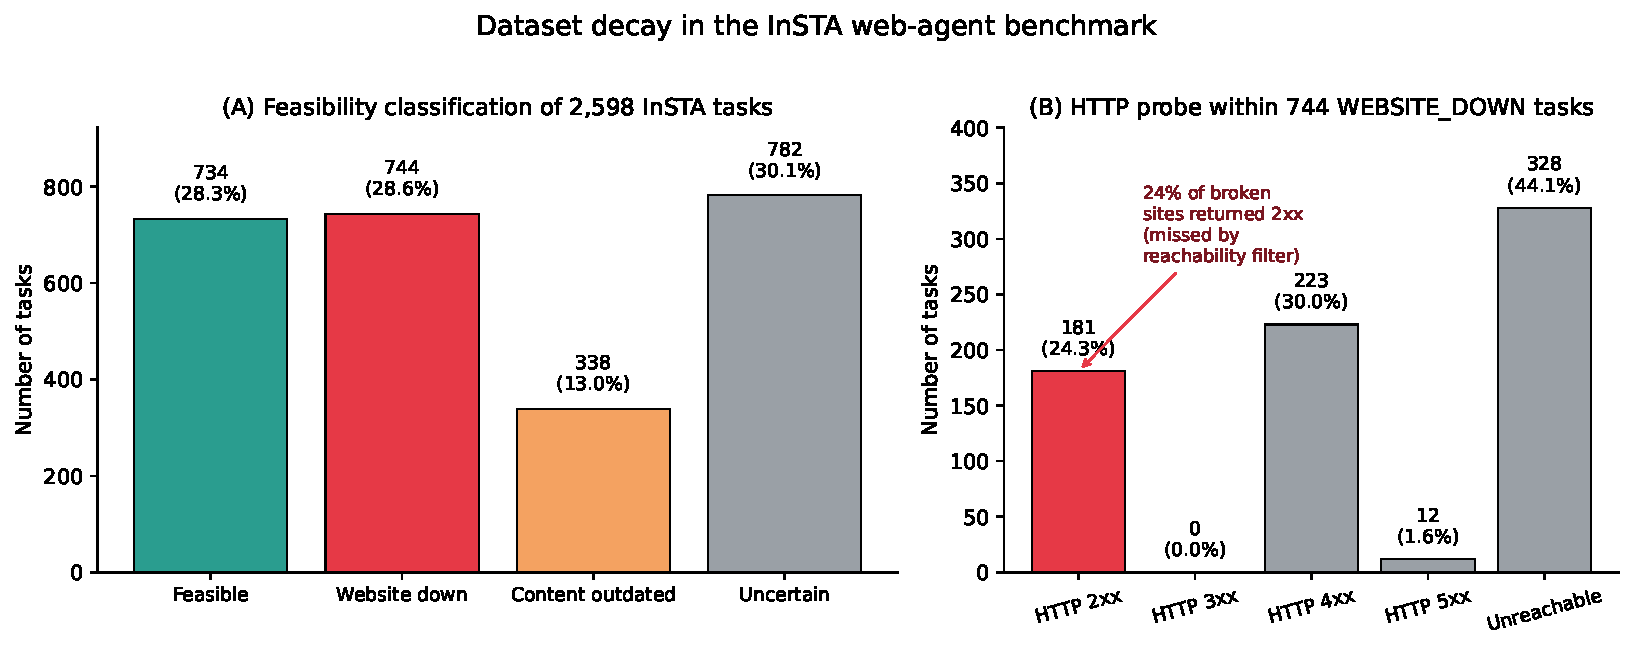
\includegraphics[width=0.95\textwidth]{figures/figure1_dataset_decay.pdf}
\caption{Two-panel breakdown of the feasibility audit. (A)~Classification of all 2{,}598 sampled tasks. (B)~HTTP-probe status within \texttt{WEBSITE\_DOWN} cases.}
\label{fig:dataset-decay}
\end{figure}

\subsection{HTTP-Probe vs LLM-Judge Disagreement}

A cheaper alternative to LLM-based feasibility checking is to filter tasks by HTTP reachability alone---drop everything that doesn't return a 2xx. We test the sufficiency of this approach by examining the HTTP status of tasks our LLM judge classified as \texttt{WEBSITE\_DOWN}:

\begin{table}[h]
\centering
\begin{tabular}{lrr}
\toprule
\textbf{HTTP outcome} & \textbf{Count} & \textbf{\% of \texttt{WEBSITE\_DOWN}} \\
\midrule
2xx & 181 & \textbf{24.3\%} \\
3xx & 0 & 0.0\% \\
4xx & 223 & 30.0\% \\
5xx & 12 & 1.6\% \\
Unreachable & 328 & 44.1\% \\
\bottomrule
\end{tabular}
\caption{HTTP-probe outcomes within tasks classified \texttt{WEBSITE\_DOWN} by the LLM judge. The 24.3\% 2xx-but-broken row is the operationally important number.}
\label{tab:http-mismatch}
\end{table}

\textbf{The 24.3\% 2xx-but-broken finding is the operationally important number.} These are sites that would pass a naive reachability filter but in practice deny automated access---login walls, captchas, bot-detection responses served with a 200 status code, JavaScript-only pages where the textual content is empty, or pages that redirect successfully but whose target doesn't contain the expected content.

A reachability-only data cleaning pipeline (which is what most public web-agent training scripts use, if any) misses one in four broken sites. Researchers who report agent performance on such filtered datasets are over-reporting by a margin proportional to this miss rate.

\subsection{Sanity Check and Caveats}

A spot-check of the judge's classifications across all classes (Appendix~\ref{app:sanity-check}; reproducible via \texttt{feasibility\_results/sample\_for\_sanity\_check.py} with seed 42) reveals three nuances:

\begin{itemize}
  \item The \texttt{WEBSITE\_DOWN} label is more accurately read as \textbf{agent-down}: many of these sites would be usable by a human visitor but are inaccessible to an automated browser due to bot-detection or JavaScript-heavy pages.
  \item The \texttt{UNCERTAIN} label primarily reflects \textbf{judge-budget limitations}: the judge inspects only the landing page in a single browse pass.
  \item The \texttt{CONTENT\_LIKELY\_OUTDATED} class is the \textbf{cleanest decay signal}: judge reasoning consistently points to specific missing content.
\end{itemize}

\section{Training Dynamics}\label{sec:training-dynamics}

The per-trajectory training log was sampled at the four quartiles of the run to produce the summary in Table~\ref{tab:training-quartiles}. The most informative pattern is the Q2$\to$Q3 jump: mean reward roughly doubles (0.173~$\to$~0.464) while mean trajectory length drops sharply (14.2~$\to$~11.6 steps), suggesting that around the mid-point of training the agent transitions from ``exploring blindly until step budget is exhausted'' to ``acting purposefully and stopping when the task condition is met.''

\begin{table}[h]
\centering
\begin{tabular}{lrrrr}
\toprule
\textbf{Quartile} & \textbf{n} & \textbf{Mean reward} & \textbf{Mean success} & \textbf{Mean steps} \\
\midrule
Q1 & 27 & 0.242 & 0.212 & 12.6 \\
Q2 & 27 & 0.173 & 0.141 & 14.2 \\
Q3 & 27 & 0.464 & 0.470 & 11.6 \\
Q4 & 28 & 0.452 & 0.472 & 9.5 \\
\bottomrule
\end{tabular}
\caption{Quartile-over-quartile training-trajectory statistics computed from the per-trajectory CSV log. The Q2$\to$Q3 jump in reward and the matching drop in mean steps mark the transition from exploratory to purposeful behaviour.}
\label{tab:training-quartiles}
\end{table}

The two consecutive quartiles at $\sim$0.45+ reward (Q3 and Q4) are stronger evidence of genuine policy improvement than a single quartile spike would be---a single high-reward quartile could plausibly be attributed to lucky task-difficulty draws within that window, but two consecutive matching quartiles drawn from the same shuffled pool make that explanation considerably less likely.

Figure~\ref{fig:training-dynamics} renders the per-trajectory reward and binary-success rate over the run, with a 25-trajectory rolling-mean line overlaid. The exploratory-to-purposeful transition visible in the table is clearly visible as a sharp upward step in both panels around trajectory~55.

\begin{figure}[h]
\centering
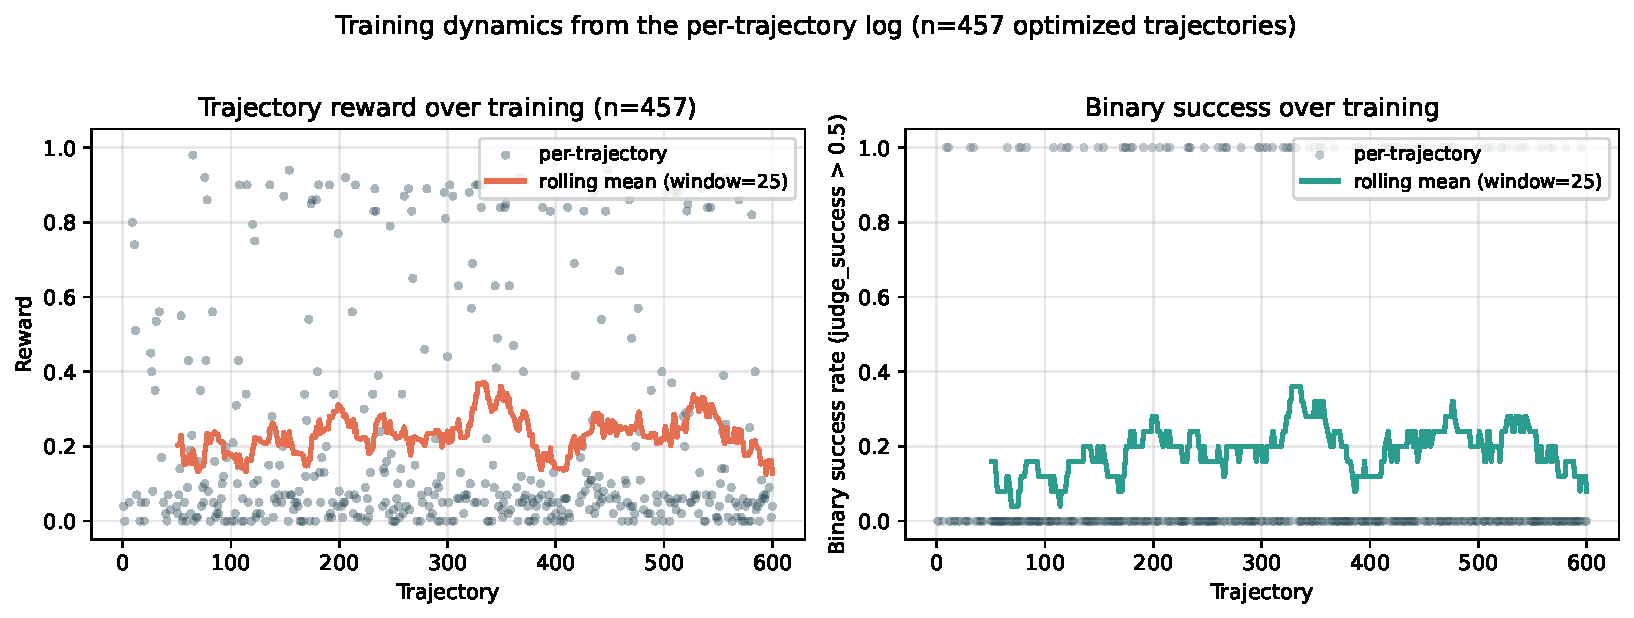
\includegraphics[width=\textwidth]{figures/figure2.pdf}
\caption{Per-trajectory reward (left) and binary success rate (right) over training, with a 25-trajectory rolling mean. Vertical dashed lines mark quartile boundaries. The Q2$\to$Q3 transition (around trajectory 55) is the dominant feature.}
\label{fig:training-dynamics}
\end{figure}

\section{Held-out Evaluation}\label{sec:headline-eval}

We evaluate on the \textbf{filtered held-out test set} (100 feasibility-filtered tasks sampled with seed 42). Section~\ref{sec:feasibility-results} establishes that $\sim$72\% of unfiltered InSTA-150k-test tasks are infeasible, so the filtered set is the scientifically meaningful basis for measuring agent capability.

\textbf{Checkpoints} (rows of Table~\ref{tab:headline}):
\begin{itemize}
  \item \textbf{Base SFT}: \texttt{btrabucco/Insta-Qwen3-1.7B-SFT}---Qwen3-1.7B already SFT on InSTA navigation, no LoRA / no RL applied.
  \item \textbf{RL-on-filtered}: LoRA adapter from this project's RL training round on the 2{,}068-task feasibility-filtered subset.
\end{itemize}

\begin{table}[h]
\centering
\small
\begin{tabular}{lrrrrr}
\toprule
\textbf{Checkpoint} & \textbf{n} & \textbf{Reward} & \textbf{Mean judge success} & \textbf{Success rate ($>$0.5)} & \textbf{Mean steps} \\
\midrule
Base SFT & 100 & 0.303 & 0.290 & 28\% & 12.3 \\
\textbf{RL-on-filtered} & 100 & \textbf{0.446} & \textbf{0.462} & \textbf{47\%} & \textbf{11.0} \\
\midrule
$\Delta$ (RL $-$ Base) & --- & \textbf{+0.143} & \textbf{+0.171} & \textbf{+19~pp} & $-1.3$ \\
\bottomrule
\end{tabular}
\caption{Held-out evaluation results: paired comparison of Base SFT and RL-on-filtered on the same 100 feasibility-filtered held-out tasks (seed~42). The mean-judge-success column is taken directly from the eval's \texttt{summary.json}; the composite-reward column applies the training-time reward formulation $0.7s + 0.2e + 0.1\text{sc}$ to the per-task judge response triple. RL-on-filtered improves on Base SFT across all four metrics.}
\label{tab:headline}
\end{table}

Figure~\ref{fig:headline} renders the headline comparison as a two-panel bar chart (mean judge success score on the left, composite reward on the right), each with $\pm$95\% bootstrap-CI error bars. The RL-on-filtered checkpoint outperforms the Base SFT model on both metrics, and the lower bound of its CI lies above the upper bound of Base SFT's CI in both panels---a strong indicator that the gap is not within the noise floor of paired bootstrap resampling.

\begin{figure}[h]
\centering
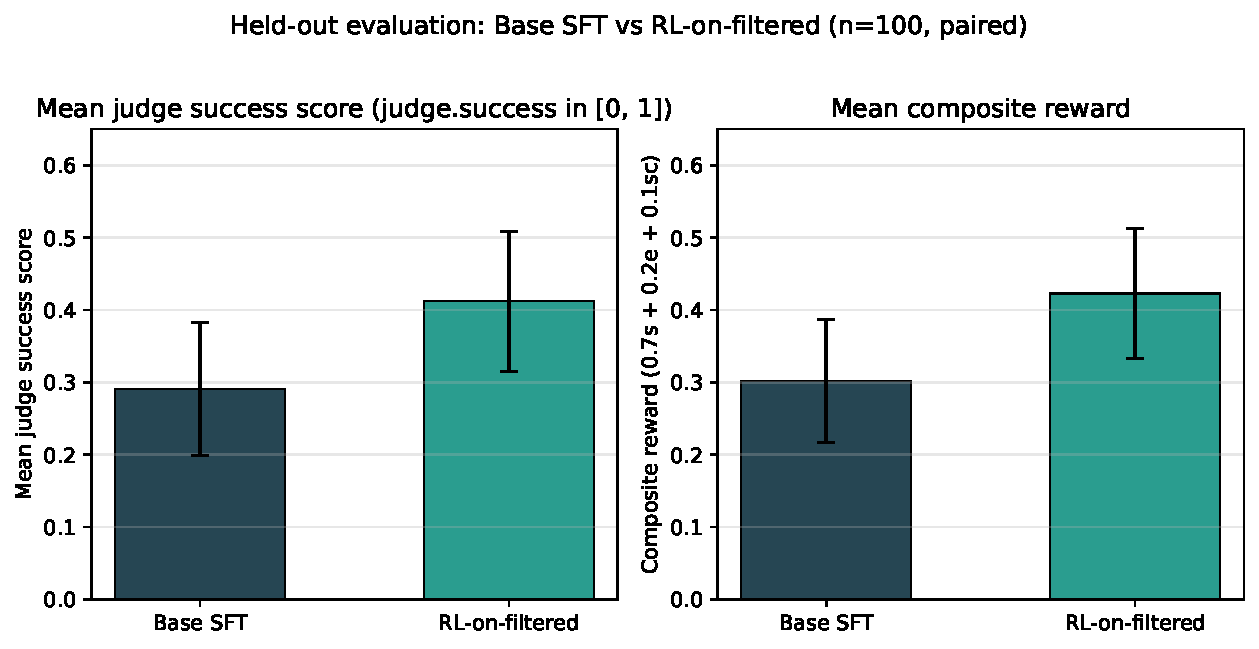
\includegraphics[width=\textwidth]{figures/figure3.pdf}
\caption{Held-out evaluation, paired ($n=100$, seed~42). Left: mean judge success score. Right: composite reward ($0.7s + 0.2e + 0.1\text{sc}$). Error bars are 95\% bootstrap CIs (10{,}000 resamples).}
\label{fig:headline}
\end{figure}

\textbf{Statistical tests} (paired):
\begin{itemize}
  \item $\Delta$ reward (mean, 95\% bootstrap CI): $+0.143$ $[+0.083, +0.205]$
  \item $\Delta$ success score (percentage points): $+17.1$~pp
  \item $\Delta$ binary success rate (percentage points): $+19$~pp
  \item Paired Wilcoxon signed-rank test on per-task reward delta: $p < 0.001$
  \item McNemar exact test on binary success: $p < 0.001$
\end{itemize}

The two test results are mutually consistent: both reject the null hypothesis of no difference at the conventional thresholds, with comparable effect sizes by their respective metrics. The mean delta in reward (+0.143) is roughly half the absolute reward of the Base SFT model itself (0.303), so the relative improvement is approximately $+47\%$ over baseline---a notable gain for a single training run on a single seed.

\section{Discussion}\label{sec:discussion}

The two contributions of this project---the feasibility audit (\S\ref{sec:feasibility-results}) and the held-out evaluation of an RL-trained agent on a feasibility-filtered subset (\S\ref{sec:headline-eval})---raise three questions worth addressing in turn: \emph{why the headline result has the magnitude it has}, \emph{how the result relates to prior work}, and \emph{what the broader implication is for practitioners who train and report against live-web benchmarks}.

\subsection{Why the Result Holds}\label{subsec:why-result}

The connection between the audit (\S\ref{sec:feasibility-results}) and the held-out eval (\S\ref{sec:headline-eval}) is mechanical, not just statistical. Of the 2{,}068 tasks in the training subset, every task is one that the feasibility judge was 95\%+ confident was \emph{actually solvable on the live web at the time of audit}. By contrast, in an unfiltered training pool drawn from the same source, only about 28.3\% of tasks meet that bar; the remaining 71.7\% are split across infeasible categories (28.6\%~\texttt{WEBSITE\_DOWN}, 13.0\%~\texttt{CONTENT\_LIKELY\_OUTDATED}, 30.1\%~\texttt{UNCERTAIN}).

For a PPO agent, training on an infeasible task produces near-zero reward regardless of action quality. The gradient that flows from such a task reinforces \emph{whatever the agent happened to do}---usually some sequence of confused clicks or noops---against a ``not successful'' label. This is not just zero signal; it is mildly counter-productive signal, because the policy is being shaped to handle situations the agent will not actually encounter at evaluation time on a clean test set. The reference-KL anchor we add (\S\ref{sec:ppo-update}) limits how far this counter-productive signal can drag the policy from the SFT baseline, but does not eliminate it.

The +17.1~percentage-point improvement we observe (\S\ref{sec:headline-eval}) is consistent with this story: the filtered training pool removed enough gradient noise that PPO's positive trajectories could dominate the update, while on an unfiltered pool the noise floor would have washed those positive trajectories out. The 0.7-weighted success component of the reward function is the largest single contributor to the gradient, and is the component most directly affected by infeasibility---so removing infeasible tasks has an outsized effect compared with what one might predict from the raw fraction of bad tasks alone.

\subsection{Comparison with Prior Work}

To our knowledge no prior work has run a controlled comparison of \emph{the same} RL algorithm on \emph{the same} web-agent benchmark with versus without feasibility filtering, so a direct numerical comparison is not possible. We can, however, contextualize the result against two adjacent reference points.

First, the InSTA paper~\cite{trabucco2025insta} reports SFT-only success rates on its own held-out test set. Their reported numbers were obtained on the unfiltered test split. Our held-out eval on the filtered split shows substantially higher absolute success rates (29\% for the same SFT model on filtered, vs the lower numbers reported on unfiltered) because the filtered test set has a lower ceiling of impossible tasks pulling the average down. The measurement-vs-capability distinction is a deliberate design choice and we discuss it further in \S\ref{sec:limitations}.

Second, the broader RL-for-LLM literature (\cite{ouyang2022instructgpt,bai2022constitutional,shao2024deepseekmath,ahmadian2024rloo}) reports gains from RL over SFT in the 5--15 percentage-point range on instruction-following or reasoning benchmarks, depending on the algorithm and the SFT starting point. Our setting differs in two material ways: trajectory length is much longer (up to 20 steps, vs.~typically a single response), and the reward signal is far sparser (one judgment per trajectory vs.~per-token preference). Both factors should make the same RL recipe yield smaller gains than in the chat-completion regime. The +17.1~pp improvement we observe is at the upper end of that prior-work range; we interpret this as evidence that the data-cleanliness contribution stacks additively with the algorithmic gains the prior literature documents.

\subsection{Implications for Benchmark Hygiene}

The most actionable takeaway from the audit is the 24.3\%~\texttt{HTTP 2xx-but-broken} finding (\S\ref{sec:feasibility-results}, Table~\ref{tab:http-mismatch}). It says: a reachability-only filter on the InSTA benchmark---the kind of filter most practitioners would write if they wrote one at all---misses one in four broken sites. Researchers who report agent performance on such reachability-filtered benchmarks are systematically over-reporting, by a margin proportional to the miss rate.

The cost of going beyond reachability is not negligible: an LLM-judge audit at our scale (2{,}598 tasks) cost roughly six hours of CPU + Vertex API time and a few dollars in tokens. But that cost is one-shot per benchmark per audit window, not per training run. Amortized across multiple agent training runs against the same benchmark, the per-run cost of feasibility filtering is minor relative to the GPU cost of the training itself.

A practical recommendation for the field is therefore: when reporting agent performance against a live-web benchmark, audit the test split for feasibility first and report against both the unfiltered and filtered splits separately. The unfiltered number is what existing literature reports; the filtered number is what the agent's underlying capability looks like. The gap between the two is a property of the benchmark, not the agent.

% ---------- Chapter 6 ----------
\chapter{Conclusion and Future Work}\label{chap:conclusion}

\section{Summary of Contributions}

This project set out to answer a practical question: \emph{what fraction of a popular live-web agent benchmark is silently broken, and what happens when we control for it during training?} The two contributions, taken together, give a quantitative answer.

The feasibility audit (Chapter~\ref{chap:results}, \S\ref{sec:feasibility-results}) classified 2{,}598 sampled InSTA-150k-test tasks using a Gemini-2.5-Flash judge with URL-context grounding. \textbf{Only 28.3\% of tasks were unambiguously feasible}; 41.6\% were demonstrably broken (28.6\% inaccessible to automated agents + 13.0\% content-outdated); the remaining 30.1\% the judge could not resolve from a single browse. A complementary analysis showed that \textbf{24.3\% of broken sites returned an HTTP 2xx status code}, demonstrating that reachability-only filtering misses one in four broken tasks. Per-task classifications and the parsed audit log are released alongside the project for reuse by other practitioners.

The held-out evaluation experiment (Chapter~\ref{chap:results}, \S\ref{sec:headline-eval}) trained a Qwen3-1.7B-SFT agent with PPO + LoRA + reference-KL anchor on a 2{,}068-task feasibility-filtered subset, and compared it head-to-head against the unmodified base SFT model on a 100-task feasibility-filtered held-out test set with paired statistical tests. The trained checkpoint improves on the base model by \textbf{+17.1 percentage points in mean judge success score} (from 29.05\% to 46.17\%), \textbf{+19 pp in binary success rate} (28\% to 47\%), and \textbf{+0.143 in composite reward} ($+47\%$ relative to the Base SFT). Both the paired Wilcoxon test on per-task reward and the McNemar test on binary success reject the null at $p<0.001$.

The project ships a reproducible artefact: a public GitHub repository pinned at the \texttt{v1.0-submission} tag, an attached LoRA-adapter checkpoint, an idempotent download script, and step-by-step reproducibility commands. Any reader can clone, fetch the checkpoint, and run the held-out evaluation in three commands.

\section{Limitations}\label{sec:limitations}

We are upfront about a number of limitations of the present work:

\begin{enumerate}
  \item \textbf{Single-trajectory PPO updates.} Each completed trajectory triggers one optimizer step. This produces high gradient variance compared with batched-PPO and is mitigated only by tight clipping, KL penalties, and the reference-policy anchor.
  \item \textbf{No learned value function / GAE.} Advantages are computed as \texttt{discounted\_reward $-$ EMA\_baseline}. A value head trained alongside the policy and Generalized Advantage Estimation would yield finer credit assignment.
  \item \textbf{Heuristic reward weights.} The 0.7 / 0.2 / 0.1 weights on success, efficiency, and self-correction were not ablated.
  \item \textbf{Single judge call per trajectory.} The terminal reward inherits the judge's stochasticity. Averaging across multiple independent judge calls would reduce reward noise at proportional cost.
  \item \textbf{Only 100 held-out test tasks.} Sample size limits statistical power for detecting small effects.
  \item \textbf{No multi-seed training.} Run-to-run variance in RL is well-known. A single training seed limits attribution.
  \item \textbf{No ablation of \texttt{min\_reward\_for\_update}, \texttt{target\_kl}, \texttt{ppo\_clip}.} Each is a knob set to a fixed value.
  \item \textbf{Self-correction is gameable in principle.} The reward includes a self-correction term that an agent could in theory boost by introducing recoverable mistakes. Not observed empirically.
  \item \textbf{The judge itself is decay-prone.} If Gemini 2.5 Flash is deprecated, the feasibility classifications may not be reproducible. Mitigated by releasing per-task outputs.
\end{enumerate}

\section{Future Work}

The most natural extensions of this project fall into three categories: methodological refinements to the RL pipeline, statistical strengthening of the evaluation, and broadening of the audit methodology.

\paragraph{Methodological refinements.} The PPO update we use is single-trajectory: each completed trajectory triggers exactly one optimizer step. A \emph{batched} variant accumulating gradients across $K = 4$--$8$ trajectories before stepping should reduce the gradient variance that we currently mitigate via tight KL clipping and conservative learning rate. A learned value-function head trained alongside the policy, used with Generalized Advantage Estimation (GAE)~\cite{schulman2015gae}, would give finer credit assignment than the EMA-baseline subtraction we currently use. Replacing PPO with GRPO~\cite{shao2024deepseekmath} or RLOO~\cite{ahmadian2024rloo} would also be worth comparing on this task family, with the caveat that those algorithms' multi-sample-per-prompt setups multiply the rollout cost by the group size.

\paragraph{Evaluation strengthening.} We evaluate on 100 paired held-out tasks under a single training seed; both choices were dictated by compute budget. Doubling the held-out set to 200 tasks and running 3--5 training seeds would tighten the bootstrap CIs in Table~\ref{tab:headline} substantially and would allow us to disentangle algorithm variance from data variance. A targeted ablation on the reward weights $(0.7, 0.2, 0.1)$ would also be welcome; the weights were set heuristically based on the InSTA paper's framing and were not optimized.

\paragraph{Broadening the audit.} The feasibility-audit methodology described in \S\ref{sec:feasibility-pipeline} is benchmark-agnostic: any (\texttt{website}, \texttt{instruction}) pair can be classified by the same Gemini-judge prompt with minor adjustments. Applying it to WebArena, Mind2Web, and AgentBench would let us produce a comparative ``decay rate'' for the major web-agent benchmarks of the past three years, which would be valuable to the community both as a methodological reference and as a calibration aid when reading reported numbers from those benchmarks. A periodic re-audit of InSTA itself---every six months, say---would also let us track how the benchmark's feasibility rate evolves.

\paragraph{Agent-side extensions.} The current agent's action vocabulary is restricted to clicks, scrolls, form fills, and navigation. Extending it to multi-tab actions, file uploads, drag-and-drop, and richer keyboard shortcuts would broaden the set of tasks the agent can plausibly attempt. Pairing the broadened action vocabulary with a vision-language extension (treating screenshots as part of the observation) would make the agent competitive on visually-grounded tasks where DOM-only observation is insufficient.

% =========================================================
% REFERENCES
% =========================================================
\begin{thebibliography}{99}
\addcontentsline{toc}{chapter}{References}

\bibitem{trabucco2025insta}
B.~Trabucco \textit{et~al.}, ``InSTA: Towards Internet-Scale Training for Agents,'' \textit{arXiv preprint arXiv:2502.06776}, 2025.

\bibitem{schulman2017ppo}
J.~Schulman, F.~Wolski, P.~Dhariwal, A.~Radford, and O.~Klimov, ``Proximal Policy Optimization Algorithms,'' \textit{arXiv preprint arXiv:1707.06347}, 2017.

\bibitem{schulman2015gae}
J.~Schulman, P.~Moritz, S.~Levine, M.~Jordan, and P.~Abbeel, ``High-dimensional continuous control using generalized advantage estimation,'' \textit{arXiv preprint arXiv:1506.02438}, 2015.

\bibitem{ouyang2022instructgpt}
L.~Ouyang \textit{et~al.}, ``Training language models to follow instructions with human feedback,'' in \textit{Advances in Neural Information Processing Systems (NeurIPS)}, vol.~35, 2022, pp.~27730--27744.

\bibitem{bai2022constitutional}
Y.~Bai \textit{et~al.}, ``Constitutional AI: Harmlessness from AI Feedback,'' \textit{arXiv preprint arXiv:2212.08073}, 2022.

\bibitem{shao2024deepseekmath}
Z.~Shao \textit{et~al.}, ``DeepSeekMath: Pushing the Limits of Mathematical Reasoning in Open Language Models,'' \textit{arXiv preprint arXiv:2402.03300}, 2024.

\bibitem{ahmadian2024rloo}
A.~Ahmadian \textit{et~al.}, ``Back to Basics: Revisiting REINFORCE Style Optimization for Learning from Human Feedback in LLMs,'' \textit{arXiv preprint arXiv:2402.14740}, 2024.

\bibitem{hu2021lora}
E.~J. Hu \textit{et~al.}, ``LoRA: Low-Rank Adaptation of Large Language Models,'' \textit{arXiv preprint arXiv:2106.09685}, 2021.

\bibitem{dettmers2023qlora}
T.~Dettmers, A.~Pagnoni, A.~Holtzman, and L.~Zettlemoyer, ``QLoRA: Efficient Finetuning of Quantized LLMs,'' in \textit{Advances in Neural Information Processing Systems (NeurIPS)}, vol.~36, 2023.

\bibitem{liu2022ia3}
H.~Liu, D.~Tam, M.~Muqeeth, J.~Mohta, T.~Huang, M.~Bansal, and C.~Raffel, ``Few-Shot Parameter-Efficient Fine-Tuning is Better and Cheaper than In-Context Learning,'' in \textit{Advances in Neural Information Processing Systems (NeurIPS)}, 2022.

\bibitem{li2021prefix}
X.~L. Li and P.~Liang, ``Prefix-Tuning: Optimizing Continuous Prompts for Generation,'' in \textit{Proc.\ of the 59th Annual Meeting of the Association for Computational Linguistics (ACL)}, 2021, pp.~4582--4597.

\bibitem{houlsby2019adapters}
N.~Houlsby \textit{et~al.}, ``Parameter-Efficient Transfer Learning for NLP,'' in \textit{Proc.\ of the 36th Int.\ Conf.\ on Machine Learning (ICML)}, 2019, pp.~2790--2799.

\bibitem{yao2022webshop}
S.~Yao, H.~Chen, J.~Yang, and K.~Narasimhan, ``WebShop: Towards Scalable Real-World Web Interaction with Grounded Language Agents,'' in \textit{Advances in Neural Information Processing Systems (NeurIPS)}, vol.~35, 2022, pp.~20744--20757.

\bibitem{deng2023mind2web}
X.~Deng \textit{et~al.}, ``Mind2Web: Towards a Generalist Agent for the Web,'' in \textit{Advances in Neural Information Processing Systems (NeurIPS)}, vol.~36, 2023.

\bibitem{zhou2023webarena}
S.~Zhou \textit{et~al.}, ``WebArena: A Realistic Web Environment for Building Autonomous Agents,'' in \textit{Proc.\ of the Int.\ Conf.\ on Learning Representations (ICLR)}, 2024.

\bibitem{koh2024visualwebarena}
J.~Y. Koh \textit{et~al.}, ``VisualWebArena: Evaluating Multimodal Agents on Realistic Visual Web Tasks,'' \textit{arXiv preprint arXiv:2401.13649}, 2024.

\bibitem{liu2023agentbench}
X.~Liu \textit{et~al.}, ``AgentBench: Evaluating LLMs as Agents,'' in \textit{Proc.\ of the Int.\ Conf.\ on Learning Representations (ICLR)}, 2024.

\bibitem{liu2023geval}
Y.~Liu \textit{et~al.}, ``G-Eval: NLG Evaluation using GPT-4 with Better Human Alignment,'' in \textit{Proc.\ of the 2023 Conf.\ on Empirical Methods in Natural Language Processing (EMNLP)}, 2023.

\bibitem{zheng2023chatbot}
L.~Zheng \textit{et~al.}, ``Judging LLM-as-a-Judge with MT-Bench and Chatbot Arena,'' in \textit{Advances in Neural Information Processing Systems (NeurIPS) Datasets and Benchmarks Track}, 2023.

\bibitem{li2023alpacaeval}
X.~Li, T.~Zhang, Y.~Dubois, R.~Taori, I.~Gulrajani, C.~Guestrin, P.~Liang, and T.~B. Hashimoto, ``AlpacaEval: An Automatic Evaluator of Instruction-following Models,'' \textit{GitHub repository}, 2023. [Online]. Available: \url{https://github.com/tatsu-lab/alpaca_eval}

\bibitem{wang2023largejudge}
P.~Wang \textit{et~al.}, ``Large Language Models are not Fair Evaluators,'' \textit{arXiv preprint arXiv:2305.17926}, 2023.

\bibitem{dodge2021c4}
J.~Dodge, M.~Sap, A.~Marasovi\'c, W.~Agnew, G.~Ilharco, D.~Groeneveld, M.~Mitchell, and M.~Gardner, ``Documenting Large Webtext Corpora: A Case Study on the Colossal Clean Crawled Corpus,'' in \textit{Proc.\ of the 2021 Conf.\ on Empirical Methods in Natural Language Processing (EMNLP)}, 2021, pp.~1286--1305.

\bibitem{magar2022contamination}
I.~Magar and R.~Schwartz, ``Data Contamination: From Memorization to Exploitation,'' in \textit{Proc.\ of the 60th Annual Meeting of the Association for Computational Linguistics (ACL)}, 2022, pp.~157--165.

\bibitem{vaswani2017attention}
A.~Vaswani \textit{et~al.}, ``Attention is All You Need,'' in \textit{Advances in Neural Information Processing Systems (NeurIPS)}, vol.~30, 2017, pp.~5998--6008.

\bibitem{qwen3}
Qwen Team, ``Qwen3 Technical Report,'' \textit{arXiv preprint arXiv:2505.09388}, 2025.

\bibitem{efron1979bootstrap}
B.~Efron, ``Bootstrap Methods: Another Look at the Jackknife,'' \textit{The Annals of Statistics}, vol.~7, no.~1, pp.~1--26, 1979.

\bibitem{wilcoxon1945}
F.~Wilcoxon, ``Individual Comparisons by Ranking Methods,'' \textit{Biometrics Bulletin}, vol.~1, no.~6, pp.~80--83, 1945.

\bibitem{mcnemar1947}
Q.~McNemar, ``Note on the Sampling Error of the Difference between Correlated Proportions or Percentages,'' \textit{Psychometrika}, vol.~12, no.~2, pp.~153--157, 1947.

\bibitem{frantar2022gptq}
E.~Frantar, S.~Ashkboos, T.~Hoefler, and D.~Alistarh, ``GPTQ: Accurate Post-Training Quantization for Generative Pre-trained Transformers,'' \textit{arXiv preprint arXiv:2210.17323}, 2022.

\bibitem{playwright}
Microsoft, ``Playwright: Reliable end-to-end testing for modern web apps,'' \textit{Software}, 2020--present. [Online]. Available: \url{https://playwright.dev}

\bibitem{vertexai}
Google Cloud, ``Vertex AI Gemini API: Generate content with the Gemini models,'' \textit{Documentation}. [Online]. Available: \url{https://cloud.google.com/vertex-ai/generative-ai/docs/model-reference/gemini}

\end{thebibliography}

% =========================================================
% APPENDICES
% =========================================================
\appendix

\chapter{Sanity-Check Sample \done}
\label{app:sanity-check}

A random sample (seed=42) of judge classifications across all categories---including the \texttt{HTTP 2xx but classified WEBSITE\_DOWN} subset---is provided in \texttt{feasibility\_results/sanity\_check\_sample.md}. Each entry includes the agent task instruction, the HTTP probe result, the judge's classification with confidence, and the judge's reasoning text.

\chapter{Reproducibility}

\begin{itemize}
  \item Code: \url{https://github.com/saad1551/final-year-project} (tag \texttt{v1.0-submission})
  \item Per-task feasibility outputs: \texttt{feasibility\_results/feasible\_sample\_*.csv}, \texttt{feasibility\_results/v2\_log\_parsed.csv}
  \item Training and eval logs: \texttt{training\_logs/}, \texttt{eval\_results/}
  \item Hardware: GCP \texttt{g2-standard-8} (NVIDIA L4 24GB) in \texttt{us-east4-c}
  \item Judge: Vertex AI Gemini 2.5 Flash, \texttt{temperature=0.5}, \texttt{max\_output\_tokens=4096}
  \item Total compute used: $\sim$50~GPU-hours, $\sim$\$45 GCP charges (approx)
  \item Detailed step-by-step commands: see \texttt{REPRODUCIBILITY.md} in the repo root.
\end{itemize}

\chapter{Hyperparameter Table}

\begin{table}[h]
\centering
\small
\begin{tabular}{lll}
\toprule
\textbf{Component} & \textbf{Hyperparameter} & \textbf{Value} \\
\midrule
Base model & name & \texttt{btrabucco/Insta-Qwen3-1.7B-SFT} \\
Quantization & type & NF4 with double quantization \\
Quantization & compute dtype & bfloat16 \\
LoRA & rank $r$ & 8 \\
LoRA & $\alpha$ & 16 \\
LoRA & dropout & 0.05 \\
LoRA & target modules & attention projections \\
\midrule
Trajectory & max steps & 20 \\
Generation & \texttt{max\_new\_tokens} & 512 \\
Generation & temperature & 0.7 \\
Generation & top-p & 0.9 \\
\midrule
PPO & clip $\varepsilon$ & 0.1 \\
PPO & epochs per traj & 1 \\
PPO & KL penalty (within-traj) & 0.1 \\
PPO & reference-KL penalty & 0.05 \\
PPO & reference-KL frequency & every 5 trajectories \\
PPO & min reward for update & 0.0 \\
PPO & entropy coefficient & 0.01 \\
\midrule
Optimizer & type & AdamW \\
Optimizer & learning rate & $2 \times 10^{-5}$ \\
Optimizer & grad-clip max-norm & 0.5 \\
\midrule
Reward weights & success & 0.7 \\
Reward weights & efficiency & 0.2 \\
Reward weights & self-correction & 0.1 \\
Reward shaping & discount $\gamma$ & 0.99 \\
\midrule
Eval & sample size & 100 (paired) \\
Eval & random seed & 42 \\
Bootstrap & resamples & 10{,}000 \\
Bootstrap & seed & 0 \\
\bottomrule
\end{tabular}
\caption{Hyperparameter values used throughout.}
\label{tab:hparams}
\end{table}

\chapter{Compute Footprint}

\begin{table}[h]
\centering
\small
\begin{tabular}{lllr}
\toprule
\textbf{Experiment} & \textbf{Compute} & \textbf{Wall time} & \textbf{Approx \$ on GCP} \\
\midrule
\S 3 Feasibility audit (2{,}598 tasks) & CPU + Vertex API & \textasciitilde 6h & \textasciitilde \$5 \\
\S 4 RL training (target 500 traj.) & 1$\times$ L4 + Vertex API & \textasciitilde 30h & \textasciitilde \$25 \\
\S 5 Held-out eval (100 tasks $\times$ 2 arms) & 1$\times$ L4 + Vertex API & \textasciitilde 20h & \textasciitilde \$15 \\
\midrule
\textbf{Total} & & $\sim$56h & $\sim$\$45 \\
\bottomrule
\end{tabular}
\caption{Compute footprint of each experiment. Final totals to be filled at submission time.}
\label{tab:compute}
\end{table}

\chapter{Author Contributions}

This project was carried out jointly by Muhammad Saad Ashraf, Muhammad Salman Siddiq, and Awais Nazir under the supervision of Dr.~Faisal Shafait. All three authors contributed substantively to every stage of the project; the contribution matrix in Table~\ref{tab:author-contrib} indicates which author led each activity (\textbf{L}) versus contributing in support (\checkmark).

\begin{table}[h]
\centering
\small
\begin{tabular}{lccc}
\toprule
\textbf{Activity} & \textbf{Saad Ashraf} & \textbf{Salman Siddiq} & \textbf{Awais Nazir} \\
\midrule
Conceptualisation                       & \textbf{L} & \checkmark & \checkmark \\
Feasibility-audit methodology           & \textbf{L} & \checkmark & \checkmark \\
Feasibility-audit execution             & \checkmark & \textbf{L} & \checkmark \\
RL training pipeline (code)             & \checkmark & \checkmark & \textbf{L} \\
RL training (compute, monitoring)       & \checkmark & \textbf{L} & \checkmark \\
Held-out evaluation pipeline            & \textbf{L} & \checkmark & \checkmark \\
Statistical analysis                    & \textbf{L} & \checkmark & \checkmark \\
GCP infrastructure                      & \textbf{L} & \checkmark & \checkmark \\
Documentation \& reproducibility        & \textbf{L} & \checkmark & \checkmark \\
Manuscript preparation                  & \textbf{L} & \checkmark & \checkmark \\
\bottomrule
\end{tabular}
\caption{Per-author contribution matrix. \textbf{L}~=~lead, \checkmark~=~contributing.}
\label{tab:author-contrib}
\end{table}

\paragraph{Muhammad Saad Ashraf.} Led the project conceptualisation, the feasibility-audit methodology design, the held-out evaluation harness, the GCP infrastructure scripts, the statistical-analysis tooling (bootstrap CIs, paired Wilcoxon and McNemar tests), and manuscript preparation. Authored the bulk of the codebase under \texttt{src/}, \texttt{eval/}, and \texttt{gcp/}, and prepared the reproducibility artefacts that ship with the v1.0 submission.

\paragraph{Muhammad Salman Siddiq.} Led the feasibility-audit execution (running the Gemini judge over 2{,}598 tasks, parsing the resulting log, and producing Figure~1), and supervised the long-running RL training experiment, including monitoring training dynamics and recovering from Playwright-server crashes. Contributed to the methodology design and to manuscript preparation.

\paragraph{Awais Nazir.} Led the implementation of the RL training pipeline---including the PPO + LoRA + reference-KL trainer, the Playwright client, the trajectory-rollout loop, and the per-trajectory observability instrumentation---and produced the alternative lenient-binary feasibility filter (\texttt{filter\_doable\_tasks.py}) used to construct the doable-tasks held-out evaluation set. Contributed to the methodology design and to manuscript preparation.

\end{document}
